%---------------------------------------------------------------------
%
%                          Cap�tulo 4
%
%---------------------------------------------------------------------
%
% 04Imagenes.tex
% Copyright 2009 Marco Antonio Gomez-Martin, Pedro Pablo Gomez-Martin
%
% This file belongs to the TeXiS manual, a LaTeX template for writting
% Thesis and other documents. The complete last TeXiS package can
% be obtained from http://gaia.fdi.ucm.es/projects/texis/
%
% Although the TeXiS template itself is distributed under the 
% conditions of the LaTeX Project Public License
% (http://www.latex-project.org/lppl.txt), the manual content
% uses the CC-BY-SA license that stays that you are free:
%
%    - to share & to copy, distribute and transmit the work
%    - to remix and to adapt the work
%
% under the following conditions:
%
%    - Attribution: you must attribute the work in the manner
%      specified by the author or licensor (but not in any way that
%      suggests that they endorse you or your use of the work).
%    - Share Alike: if you alter, transform, or build upon this
%      work, you may distribute the resulting work only under the
%      same, similar or a compatible license.
%
% The complete license is available in
% http://creativecommons.org/licenses/by-sa/3.0/legalcode
%
%---------------------------------------------------------------------

\chapter{Implementaci\'on y Especificaci\'on}
\label{cap4}
\label{cap:implentacion-especificacion}


\begin{FraseCelebre}
\begin{Frase}
%El alma nunca piensa sin una imagen mental.
\end{Frase}
\begin{Fuente}
%Arist�teles
\end{Fuente}
\end{FraseCelebre}

%-------------------------------------------------------------------
\section{Introducci\'on}
%-------------------------------------------------------------------
\label{cap4:sec:intro}

Una vez decididas las herramientas que se iban a usar y con gran parte de la informaci\'on recogida, lleg\'o el momento de realizar un an\'alisis del funcionamiento de Android y dise\~nar un protocolo de red que ayudase a conectar la aplicaci\'on de Android con el juego de Unity. En este cap\'itulo se explicar\'an todas las decisiones que se tomaron a la hora de implementar ambas aplicaciones y se ampliar\'a la informaci\'on sobre como interactuan ambos sistemas.

%-------------------------------------------------------------------
\section{Arquitectura global}
%-------------------------------------------------------------------
\label{cap4:sec:global}

Tal y como se ha planteado en los anteriores cap\'itulos, para la realizaci\'on de este proyecto se ha requerido de la conexi\'on entre una aplicaci\'on de escritorio realizada con Unity3D y una aplicaci\'on de un dispositivo m\'ovil Android. Ambos dispositivos recibir\'an y enviaran mensajes pero el protocolo a seguir ha sido UDP. UDP es un protocolo a nivel de transporte que permite el env\'io de datagramas a trav\'es de la red sin necesidad de haber realizado una conexi\'on previa. Esto se consigue gracias a que la cabecera del propio datagrama UDP incorpora la informaci\'on suficiente para realizar su direccionamiento.
\\
Con la utilizaci\'on de UDP se corre el riesgo de p\'erdida de informaci\'on, cosa que para este proyecto es menos probable ya que en ning\'un momento este datagrama sale a internet. Se ha puesto como requisito que tanto el ordenador como el dispositivo m\'ovil se encuentren conectados a la misma red local, lo que hace muy poco probable la p\'erdida de paquetes UDP. Esta posible p\'erdida ser\'a analizada en el cap\'itulo siguiente donde se analiza las pruebas realizadas con usuarios.
\\


A la hora de iniciar la conexi\'on, es la aplicaci\'on m\'ovil la que va a conectarse al puerto que abra la aplicaci\'on de escritorio previamente. Para poder hacer esto, se propuso la utilizaci\'on de un QR. Este QR contiene la informaci\'on de la IP del ordenador donde se est\'a ejecutando el juego y el puerto designado para la recepci\'on de los mensajes provenientes de la aplicaci\'on m\'ovil. Una vez la aplicaci\'on m\'ovil guarda esos datos extraidos tras leer el c\'odigo QR, se incia la conexi\'on y el intercambio de paquetes entre ambas aplicaciones.
\\
La decisi\'on de usar UDP cobr\'o su importancia en este apartado ya que no se espera un intercambio ordenado de informaci\'on entre ambas aplicaciones ,ya que el usuario puede hacer una pulsaci\'on en la pantalla del m\'ovil en cualquier momento. La informaci\'on que se env\'ia desde la aplicaci\'on Android es la siguiente:

\begin{enumerate}

\item Dimensiones de la pantalla del dispositivo m\'ovil con 2 enteros, ancho y alto.
\item Pulsaci\'on en la pantalla con 3 enteros (X, Y, tipo de evento). 

\end{enumerate}

Las dimensiones se mandan \'unicamente una vez al iniciar la conexiones mientras que las coordenadas de las pulsaciones se env\'ian cada vez que estas ocurren. El tercer entero que se manda en estos paquetes viene definido por cada tipo de pulsaci\'on que se puede registrar en Android. Los tipos contemplados son:
\begin{itemize} 
\item \textbf{ACTION\_DOWN:} Env\'ia el valor 0. Este evento se dispara al realizar una pulsaci\'on en la pantalla.
\item \textbf{ACTION\_UP:} Env\'ia el valor 2. Este evento se dispara al levantar el dedo de la pantalla.
\end{itemize}

En el lado del servidor de la aplicaci\'on de Unity se espera la llegada de las dimensiones de la pantalla que env\'ia la aplicaci\'on m\'ovil para enviar desde su lado la siguiente informaci\'on en paquetes diferentes:

\begin{enumerate}
\item Tiempo de vibraci\'on que debe realizarse cada vez que se pulse una posici\'on correcta de la pantalla del m\'ovil. Se considera una pulsaci\'on correcta un punto que est\'e dentro de un bot\'on.
\item Imagen del mando con o sin fondo cogido directamente de una c\'amara de Unity.
\item En caso de que el juego admita la vibraci\'on del m\'ovil, se env\'ia la acci\'on de realizar la vibraci\'on o no.
\end {enumerate}

El primero de estos mensajes con el tiempo de vibraci\'on solamente se env\'ia una \'unica vez al inicio de la conexi\'on.
\\
El flujo de mensajes durante la ejecuci\'on de estas aplicaciones tiene un intercambio de datagramas constante de \'ordenes para que el dispositivo m\'ovil vibre, im\'agenes compridas y coordenadas de pulsaciones de la pantalla del dispositivo m\'ovil.
La figura XXXX describe este protocolo de manera m\'as gr\'afica.

\begin{figure}[h]
\centering
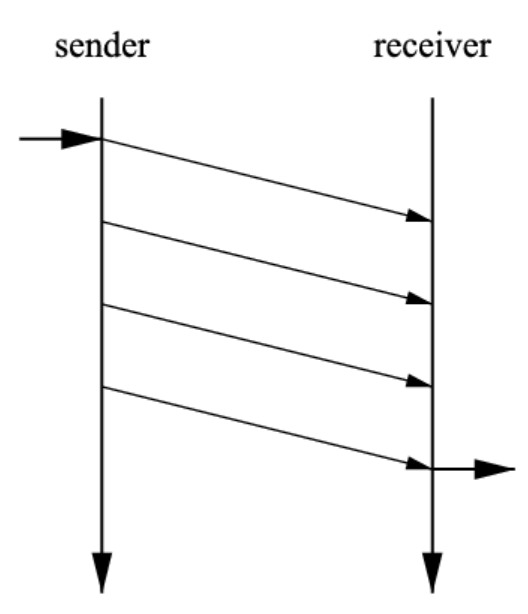
\includegraphics[width=0.6\textwidth]{Imagenes/Bitmap/UDP-protocol.png}
\caption{Protocolo de comunicaci\'on entre las aplicaciones}
\label{Protocolo Android - Unity}
\end{figure}

\newpage
%-------------------------------------------------------------------
\section{Aplicaci\'on m\'ovil}
%-------------------------------------------------------------------
\label{cap4:sec:android}

La principal funci\'on de este proyecto es el uso de un dispositivo Android para controlar de manera remota un videojuego realizado en Unity. Para esto es necesario conocer la arquitectura de Android y c\'omo funciona el ciclo de vida de sus aplicaciones.
La siguiente figura muestra el ciclo de vida de cualquier aplicaci\'on que se ejecute en un dispositivo Android.
\\
\begin{figure}[h]

\centering
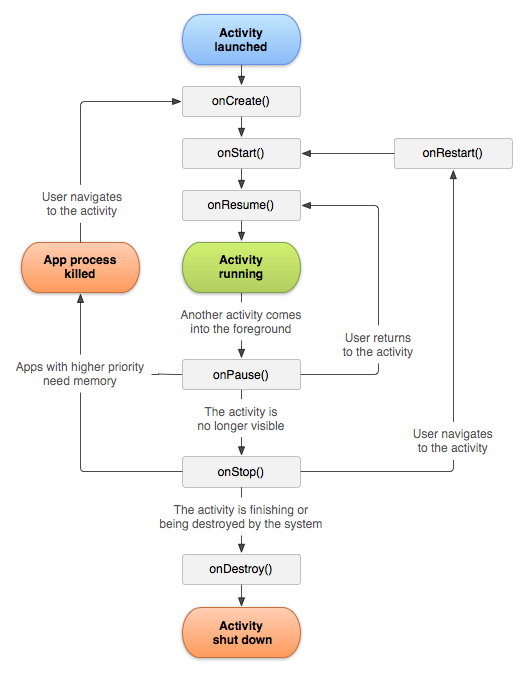
\includegraphics[width=0.6\textwidth]{Imagenes/Bitmap/Ciclo_de_vida_Android.png}
\caption{Ciclo de Vida de una Actividad de Android}
 \label{Ciclo de vida android}
\end{figure}
\\
Como puede observarse, cada Activity de una aplicaci\'on ejecutada en Android tiene varias etapas por las que puede pasar:

\begin{enumerate}
\item onCreate()
\item onStart()
\item onResume()
\item onPause()
\item onStop()
\item onDestroy()
\end {enumerate}

Cuando el usuario comienza a abandonar la actividad, el sistema llama a m\'etodos para desmantelarla. En algunos casos, este desmantelamiento es solo parcial ya que la actividad todav\'ia reside en la memoria (por ejemplo, cuando el usuario cambia a otra app) y a\'un puede volver al primer plano. En caso de que el usuario vuelva a poner dicha actividad en primer plano, esta se reanuda donde el usuario la dej\'o.
\\
Adem\'as de ciclo de vida, Android tiene un sistema de permisos. Desde la versi\'on 6.0 de Android (nivel de API 23) pueden incluirse en el fichero de manifiesto de la app los permisos que se deben solicitar al usuario para poder acceder a algunos recursos espec\'ificos. En este proyecto se necesita usar la c\'amara para poder realizar la lectura del c\'odigo QR, es por esto que se ha tenido que a\~nadir este permiso en el fichero de manifiesto de la app.
\\
Este c\'odigo QR es generado gracias a la librer\'ia de ZXing.NET desde la aplicaci\'on de Unity, la cual se cuenta en la siguiente secci\'on. Android por su parte incorpora una API para la lectura de c\'odigos. El c\'odigo QR contiene la siguiente informaci\'on:

\begin{itemize}
\item IP del servidor donde se est\'a ejecutando el juego.
\item Puerto de escucha del servidor.
\end {itemize}

Si el c\'odigo QR que se lee es correcto, se lanza una segunda Activitidad. La creaci\'on de una segunda actividad permite usar un archivo de manifiesto diferente y con \'el, generar una interfaz de usuario adecuada a esta segunda actividad. Esta segunda actividad tiene como prop\'osito establecer la comunicaci\'on con el servidor ya iniciado en la direcci\'on IP extraida del c\'odigo QR y a su vez el intercambio de informaci\'on (pulsaciones e im\'agenes) durante la sesi\'on de juego.
\\
\begin{figure}[h]
\centering
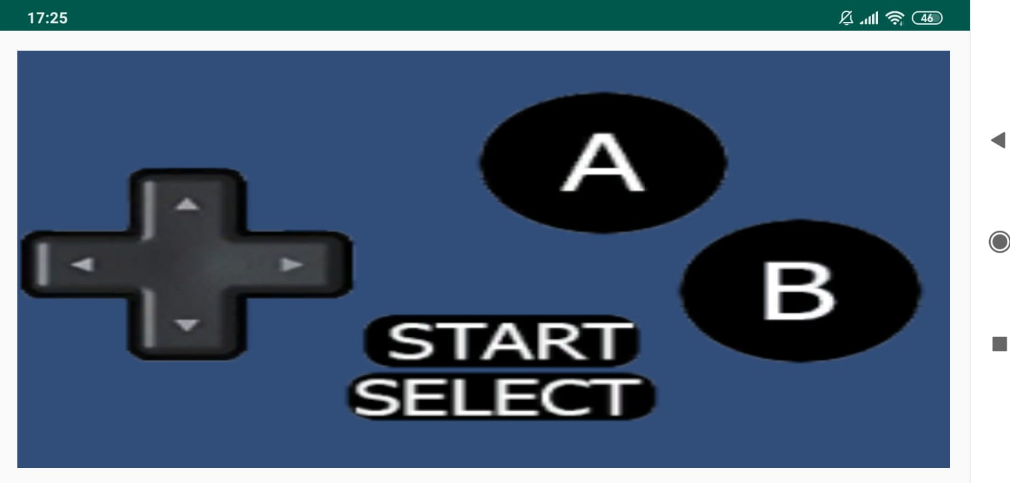
\includegraphics[width=0.8\textwidth]{Imagenes/Bitmap/Mando.png}
\caption{Vista del mando enviado desde Unity a Android}
 \label{Mando}
\end{figure}
\\
En caso de que el c\'odigo QR se lea correctamente, se inciar\'a la conexi\'on con el servidor que se est\'a ejecutando en Unity. En el siguiente apartado se explica la ejecuci\'on en la lado de Unity y el inicio de la conexi\'on con este. Desde Unity se env\'ia de manera constanste un streaming de im\'agenes sacadas de una c\'amara auxiliar colocada en la escena del juego. Esto permite en el env\'io de tanto un mando, mando con gameplay o \'unicamente gameplay. Para la demostraci\'on de este proyecto, se ha optado por el env\'io de la im\'agen de un mando de manera exclusiva. Este mando puede verse en la figura XXXXX . 
\\

Esta im\'agen llega al dispositivo Android tras realizarse una compresi\'on a formato PNG en el lado del servidor. Los bytes que llegan son convertidos a un tipo Bitmap y este Bitmap es usado como fondo de la Actividad. Este proceso se realiza constantemente ya que en caso de que se quiera utilizar para gameplay, este vaya fluido. En el cap\'ítulo siguiente se tratan las pruebas con usuario donde se hace un estudio de cu\'anto tarda esta im\'agen en procesarse y enviarse. 
\\
La arquitectura de este proyecto de Android puede verse en la figura XXXX. 
\\
\begin{figure}[h]
\centering
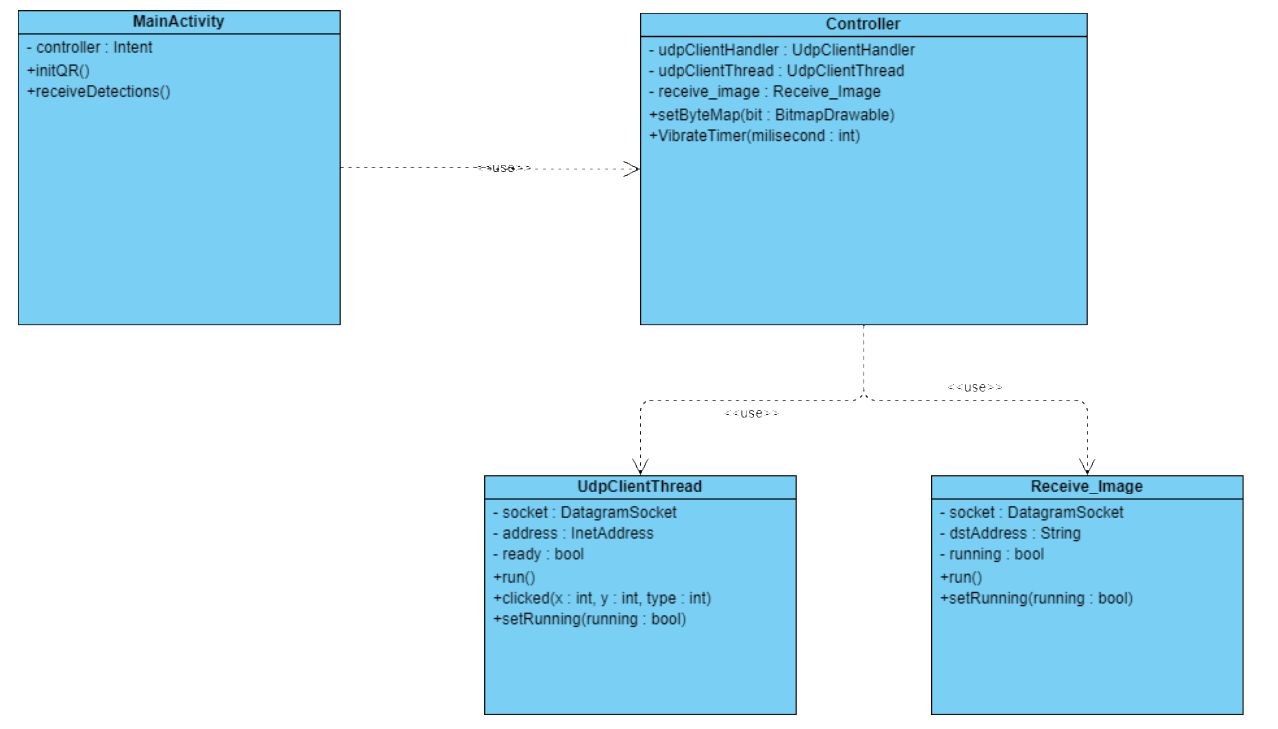
\includegraphics[width=1.0\textwidth]{Imagenes/Bitmap/Arquitectura_Android.png}
\caption{Arquitectura de la aplicaci\'on Android}
 \label{Arquitectura_Android}
\end{figure}
\\

\textbf{MainActivity} y \textbf{Controller} son las 2 actividades que se ha comentado anteriormente que existen en este proyecto de Android. La funci\'on de MainActivity es la de la lectura del QR. Su dise\~no tiene como \'unico prop\'osito el de mostrar la c\'amara para la lectura del QR. Se encarga de pedir los permisos necesarios para el uso de la c\'amara. Cuando el QR es correcto, guarda la informaci\'on y antes de terminar ordena la creaci\'on de una segunda actividad con la informaci\'on del QR. La informaci\'on del QR es de tipo \textbf{String} y tiene como formato \textit{IP:Puerto}. 
\\
Adem\'as de la informaci\'on del QR y las im\'agenes, hay otro dato que interviene en la comunicaci\'on entre las 2 aplicaciones planteadas para este proyecto. Estos datos son las pulsaciones de la pantalla del dispositivo Android. En estos mensajes se env\'ian los datos de las coodenadas (x,y) donde el usuario ha pulsado y adem\'as el tipo de gesto que ha hecho (pulsar o levantar). La disposici\'on de los bytes que se env\'ian puede verse en la figura XXX. Un mensaje que \'unicamente se realiza al inicio de la conexi\'on es el del env\'io de las dimensiones de la pantalla que tiene el dispositivo Android. La disposici\'on de los bytes de este mensaje puede verse en la figura XXX.


\newpage
%-------------------------------------------------------------------
\section{Aplicaci\'on PC}
%-------------------------------------------------------------------
\label{cap4:sec:aplicaiconPC}



% Variable local para emacs, para  que encuentre el fichero maestro de
% compilaci�n y funcionen mejor algunas teclas r�pidas de AucTeX
%%%
%%% Local Variables:
%%% mode: latex
%%% TeX-master: "../ManualTeXiS.tex"
%%% End:
